\section{Simulation Study}
\label{simulation}

As the ensemble data described in \cref{case} cannot be published we instead provide a simulated exampel, with an identical framework.

\subsection{The Data}

The simulation data uses an identical set to the case data, 4 zones with different production capacity. The observational data is reused and thus identical to the case.

To replace the ensambles we simulated en ornstein-uhlenbeck (OU) mean-reverting process

\begin{equation}
    dX = \kappa\big(\mu(t) - X\big)\,dt + \sigma\, dB_t, 
    \qquad j = 1,\dots,n_{\mathrm{ensembles}}.
\end{equation}

The process was driven using the actual observations at each timepoint, scaled to the interval $\mu(t) = \frac{y_t}{c_{zone}}, \, c_{zone = \max y_t} $ Scaling was done simply to streamline the simulation code and allow parameters to be chosen independently of zones.

Simulation was performed using a euler-maruyama scheme, with timesteps of $dt = 1$. afterwards simulated ensembles were scaled back to original scale. 
\begin{equation}
    X_t = X_{t-1} + \kappa(\mu_{t} - X_{t-1}) + \sigma\epsilon_t
\end{equation}

where $\epsilon_t \sim N(0,1)$ and IID.

For this simulation study the parameters $\kappa = 0.33$ and $\sigma = 0.033$ was chosen.


\subsection{Procedure}

The procedure used to analise the simulation example is identical to the one used in \cref{case} for detail refer to this chapter.

\subsection{results}

An example of the forecast provided by the method can be seen in \cref{fig:forecastexample}. Where the correlation corrected forecast is provided. The period visualised is the same as in \cref{fig:casedata} for comparison purpose.

\begin{figure}
    \centering
    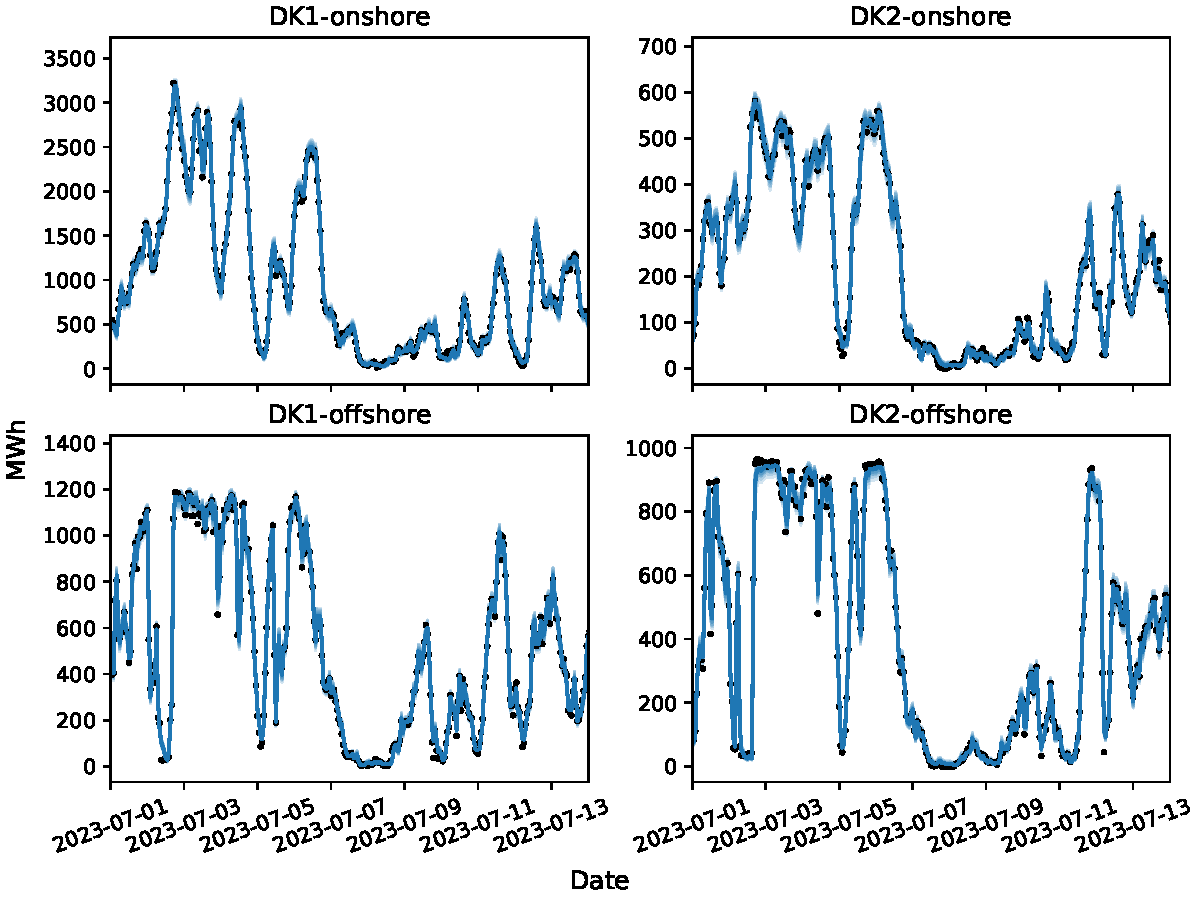
\includegraphics[width=1\linewidth]{Results/Graphs/corrolation_example_sim.pdf}
    \caption{Caption}
    \label{fig:forecastexample}
\end{figure}

The loss curves during the training of the neural nets can be seen in \cref{fig:loss}. Showing both the training and validation loss.

\begin{figure}
    \centering
    \includegraphics[width=1\linewidth]{Results/Graphs/loss_curves_sim.pdf}
    \caption{Caption}
    \label{fig:loss}
\end{figure}

To inform SARIMA model structure. The ACF and PACf for the pseudoresiduals are plotted in \cref{fig:acf_pacf} both before an after applying the correlation models.

\begin{figure}
    \centering
    \includegraphics[width=1\linewidth]{Results/Graphs/acf_pacf_sim.pdf}
    \caption{Caption}
    \label{fig:acf_pacf}
\end{figure}


For the SARIMA models the estimated parameters are found in \cref{tab:parameters}. Where parameters estimated using both the simple- and latent model are presented.

\begin{tabular}{lrrrrrrrr}
\toprule
 & \multicolumn{2}{r}{DK1-onshore} & \multicolumn{2}{r}{DK2-onshore} & \multicolumn{2}{r}{DK1-offshore} & \multicolumn{2}{r}{DK2-offshore} \\
 & Latent & Simple & Latent & Simple & Latent & Simple & Latent & Simple \\
\midrule
$\\theta_1$ & 0.19 & 0.30 & 0.55 & 0.42 & 0.44 & 0.75 & 0.56 & 0.78 \\
\cline{1-9}
$\\phi_1$ & 0.24 & 0.17 & -0.05 & -0.05 & -0.05 & -0.40 & -0.07 & -0.19 \\
\cline{1-9}
$\\Theta_1$ & 0.02 & 0.02 & 0.01 & 0.01 & 0.03 & 0.02 & 0.01 & 0.00 \\
\cline{1-9}
$\\sigma^2$ & 0.63 & 0.64 & 0.66 & 0.60 & 0.53 & 0.59 & 0.70 & 0.57 \\
\cline{1-9}
\bottomrule
\end{tabular}


The finally performance metrics for all zones and models are presented in \cref{tab:scores}. showing the raw ensemble scores, as well as model scores as a percentage of the ensemble scores.

\begin{table}[htb]
\centering
\caption[Ensemble summary]{Model Scores (Ensemble in Original Units; Other Models as Percent of Ensemble)}
\label{tab:ensemble_combined}
\begin{tabular}{llrrrr}
\toprule
 &  & MAE & RMSE & CRPS & VarS \\
\midrule
\multirow[c]{5}{*}{DK1-onshore} & Ensembles & 325.60 & 439.79 & 236.15 & 68.71 \\
\cline{2-6}
 & Simple - Marginal & \bfseries 36.7\% & \bfseries 36.7\% & \bfseries 40.6\% & \bfseries 78.6\% \\
\cline{2-6}
 & Latent - Marginal & \bfseries 32.0\% & \bfseries 32.6\% & \bfseries 33.1\% & \bfseries 45.1\% \\
\cline{2-6}
 & Simple & \bfseries 36.6\% & \bfseries 36.7\% & \bfseries 37.8\% & \bfseries 43.9\% \\
\cline{2-6}
 & Latent & \bfseries 32.0\% & \bfseries 32.5\% & \bfseries 32.5\% & \bfseries 35.0\% \\
\cline{1-6} \cline{2-6}
\multirow[c]{5}{*}{DK2-onshore} & Ensembles & 62.57 & 83.80 & 44.45 & 13.29 \\
\cline{2-6}
 & Simple - Marginal & \bfseries 37.3\% & \bfseries 37.7\% & \bfseries 41.0\% & \bfseries 73.5\% \\
\cline{2-6}
 & Latent - Marginal & \bfseries 37.4\% & \bfseries 37.5\% & \bfseries 39.3\% & \bfseries 52.2\% \\
\cline{2-6}
 & Simple & \bfseries 37.4\% & \bfseries 37.8\% & \bfseries 40.6\% & \bfseries 61.9\% \\
\cline{2-6}
 & Latent & \bfseries 37.4\% & \bfseries 37.6\% & \bfseries 39.7\% & \bfseries 46.6\% \\
\cline{1-6} \cline{2-6}
\multirow[c]{5}{*}{DK1-offshore} & Ensembles & 158.79 & 206.86 & 110.34 & 35.17 \\
\cline{2-6}
 & Simple - Marginal & \bfseries 43.6\% & \bfseries 45.3\% & \bfseries 48.4\% & \bfseries 72.0\% \\
\cline{2-6}
 & Latent - Marginal & \bfseries 42.9\% & \bfseries 44.4\% & \bfseries 45.5\% & \bfseries 61.1\% \\
\cline{2-6}
 & Simple & \bfseries 43.6\% & \bfseries 45.3\% & \bfseries 47.2\% & \bfseries 55.3\% \\
\cline{2-6}
 & Latent & \bfseries 42.9\% & \bfseries 44.4\% & \bfseries 45.1\% & \bfseries 50.5\% \\
\cline{1-6} \cline{2-6}
\multirow[c]{5}{*}{DK2-offshore} & Ensembles & 131.31 & 173.00 & 91.49 & 32.27 \\
\cline{2-6}
 & Simple - Marginal & \bfseries 42.0\% & \bfseries 44.6\% & \bfseries 45.8\% & \bfseries 60.8\% \\
\cline{2-6}
 & Latent - Marginal & \bfseries 39.5\% & \bfseries 41.9\% & \bfseries 41.6\% & \bfseries 49.3\% \\
\cline{2-6}
 & Simple & \bfseries 42.1\% & \bfseries 44.6\% & \bfseries 45.4\% & \bfseries 48.9\% \\
\cline{2-6}
 & Latent & \bfseries 39.5\% & \bfseries 41.9\% & \bfseries 41.6\% & \bfseries 43.5\% \\
\cline{1-6} \cline{2-6}
\bottomrule
\end{tabular}
\end{table}
